\section{Anwendungen der ZRD}

\subsection{Lösung der ZRD im Zeitbereich}{176-180}
\label{ZRD Lösung Zeitbereich}


Durch eine Transformation der ZRD in den Frequenzbereich, algebraische Berechnungen und anschliessender Rücktransformation in den Zeitbereich
ergibt sich die \textbf{Lösung der ZRD im Zeitbereich} als:

\vspace{-0.2cm}

\begin{empheq}[box=\fbox]{align*}
    x(t) &= \underbrace{ e^{\bm{A} t} \cdot x_0}_{x_F} + \underbrace{ \int\limits_0^t e^{\bm{A} (t - \tau)} \cdot \bm{B} \cdot u(\tau) \, \diff \tau }_{x_E} \\
    y(t) &= \underbrace{ \bm{C} \cdot e^{\bm{A} t} \cdot x_0 }_{y_F} + \underbrace{ \bm{C} \cdot \int\limits_0^t  \e^{\bm{A} (t - \tau)} \cdot \bm{B} \cdot u(\tau) \, \diff \tau + \bm{D} \cdot u(t)}_{y_E}
\end{empheq}


\begin{tabular}{ll}
    $x_F$   & Freie Antwort: System mit $u = 0$ aus Anfangszustand $x_0 = x(0)$ loslassen   \\
    $x_E$   & Erzwungene Antwort: System aus Zustand $x_0 = 0$ loslassen                    \\
            & \textrightarrow\ nur abhängig von Eingangssignal $u$
\end{tabular}

\smallskip

\textbf{Hinweis:} $e^{\bm{A} t} = \bm{\Phi}(t)$ heisst \textbf{Transitionsmatrix} \textrightarrow\ siehe Abschnitt \ref{Transitionsmatrix}

\medskip


\paragraph{Eigenschaften -- Freie Antwort}

Für die freie Antwort ergeben sich aus der Theorie der Eigenwerte / Eigenvektoren die folgenden Eigenschaften:

\begin{outline}
    \1 Zeigt der Startwert $x_0 = v_i$ in die Richtung eines Eigenvektors, so bewegt sich der Zustand ausschliesslich in diese Richtung:
        $x(t) = e^{\lambda_i t} \cdot v_i = e^{\lambda_i t} \cdot x_0$
    \1 Zeigt $x_0$ in eine beliebige Richtung, so kann $x(t)$ durch Superposition bestimmt werden
        \2 $x_0$ wird in Richtung der Eigenvektoren $v_i$ zerlegt und jede dieser Komponenten folgt bei der zeitlichen Entwicklung dem Faktor $e^{\lambda_i t}$
\end{outline}



\subsubsection{Impulsantwort $\boldsymbol{g(t)}$}

Ist die Transitionsmatrix $e^{\bm{A} t} = \bm{\Phi}(t)$ bekannt, so ist die \textbf{Impulsantwort $g(t)$}
$$ \boxed{ g(t) = \bm{C} \cdot e^{\bm{A} t} \cdot \bm{B} + \bm{D} \cdot \delta(t) = \bm{C} \cdot \bm{\Phi}(t) \cdot \bm{B} + \bm{D} \cdot \delta(t) } $$


\subsection[Transitionsmatrix]{Transitionsmatrix $e^{\bm{A} t} = \bm{\Phi}$}{177}
\label{Transitionsmatrix}

\begin{minipage}[c]{0.7\columnwidth}
    \raggedright
    Die Transitionsmatrix (auch Fundamentalmatrix genannt) ist (wie oben bereits angewandt) definiert als:
\end{minipage}
\hfill
\begin{minipage}[c]{0.28\columnwidth}
    \raggedright
    $$ \boxed{ e^{\bm{A} t} = \bm{\Phi}(t) } $$
\end{minipage}

\smallskip

Sie wird benötigt, um die Zustandsraumdarstellung im \textbf{Zeitbereich} zu lösen.
Es gibt grundsätzlich mehrere Methoden, die quadratische $(n \times n)$ Transitionsmatrix zu bestimmen.

\smallskip

Hier soll allerdings die analytische Berechnung mittels inverser Laplace-Transformation erwähnt sein:
$$ \boxed{ \bm{\Phi}(t) = e^{\bm{A} t} = \mathcal{L}^{-1} \Bigl\{ (s \bm{I} - \bm{A})^{-1} \Bigr\} } $$

\textbf{Hinweis:} Die Rücktransformation erfolgt erst im letzten Schritt. \\
\textrightarrow\ Jedes Element der Matrix wird \textbf{einzeln} rücktransformiert


\medskip

\paragraph{Eigenschaften der Transitionsmatrix $\bm{\Phi}(t) = e^{\bm{A} t}$}

\smallskip

\begin{ctabular}{c | c | c}
    $\bm{\Phi}(0) = \bm{I}$ & $\bm{\dot{\Phi}}(t) = \bm{A} \cdot \bm{\Phi}(t) \, (= \bm{\Phi}(t) \cdot \bm{A})$ & $\bm{\Phi}(t)$ ist stets invertierbar
\end{ctabular}



\paragraph{Transitionsmatrix einer Diagonalmatrix}

Die Transitionsmatrix $\bm{\Phi}(t) = e^{\bm{A} t}$ kann eifach berechnet werden, wenn $\bm{A}$ eine Diagonalmatrix ist.

$$
\bm{A_{\rm Diag}} = 
\begin{bmatrix}
    \lambda_1   & 0     \\
    0           & \lambda_2 
\end{bmatrix} 
\qquad \Rightarrow\ \quad
e^{\bm{A_{\rm Diag}} t} = 
\begin{bmatrix}
    e^{\lambda_1 t} & 0                 \\
    0               & e^{\lambda_2 t}
\end{bmatrix} 
$$

\textbf{Hinweis:} Diagonalisierung einer Matrix: siehe Abschnitt \ref{Diagonalisierung}


\subsection{Entkopplung mittels Diagonalform}{180-185}

Die Diagonalform entkoppelt die $n$ Differentialgleichunge 1. Ordnung der ZRD, sodass man $\bm{n}$ \textbf{voneinander unabhängige} Differentialgleichungen erhält.

\smallskip

Die Lösung der Zustandsgleichungen (bzw. der ZRD) ist besonders einfach, wenn sich das System in \textbf{Diagonalform} befindet.
Ausserdem ist die \textbf{Stabilität} des Systems sofort an der \textbf{Diagonalmatrix} $\bm{\Lambda} = \bm{A_{\rm Diag}}$ ablesbar.

\smallskip

Für ein \textbf{SISO-System} ist die Diagonalform gegeben als:


\begin{minipage}[t]{0.5\columnwidth}
    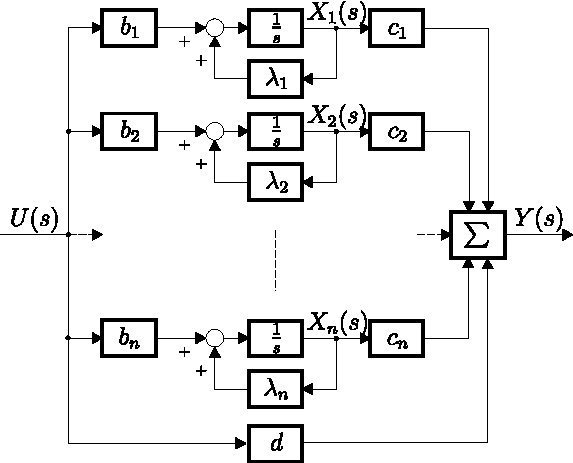
\includegraphics[width=\columnwidth, align=t]{images/ZRD_diagonalform.pdf}
\end{minipage}
\hfill
\begin{minipage}[t]{0.48\columnwidth}

    \vspace{-0.2cm}

    $$
    \begin{bmatrix}
        \dot{x}_1 \\
        \dot{x}_2 \\
        \vdots \\
        \dot{x}_n
    \end{bmatrix}
    =
    \overbrace{
    \begin{bmatrix}
        \lambda_1   & 0         & \cdots    & 0         \\
        0           & \lambda_2 & \ddots    & \vdots    \\
        \vdots      & \ddots    & \ddots    & 0         \\
        0           & 0         & \cdots    & \lambda_n
    \end{bmatrix}
    }^{\bm{\Lambda} = \bm{A_{\rm Diag}}}
    \begin{bmatrix}
        x_1 \\
        x_2 \\
        \vdots \\
        x_n
    \end{bmatrix}
    +
    \begin{bmatrix}
        b_1 \\
        b_2 \\
        \vdots \\
        b_n
    \end{bmatrix}
    \cdot u
    $$
    $$
    y =
    \begin{bmatrix}
        c_1 & c_2 & \dots & c_n
    \end{bmatrix}
    \cdot
    \begin{bmatrix}
        x_1 \\
        x_2 \\
        \vdots \\
        x_n
    \end{bmatrix}
    + d \cdot u
    $$
\end{minipage}
    

Aus dem Diagramm ist ersichtlich, dass das System folgende UTF $G(s)$ hat:

$$ G(s) = \frac{Y(s)}{U(s)} = \frac{b_1 c_1}{s - \lambda_1} +  \frac{b_2 c_2}{s - \lambda_2} + \cdots + \frac{b_n c_n}{s - \lambda_n} $$


\paragraph{Eigenschaften der Diagonalform}

\begin{outline}
    \1 Wenn $G(s)$ \textbf{minimal} ist, entsprechen die Diagonal-Elemente $\lambda_i$ der Systemmatrix $\bm{\Lambda} = \bm{A_{\rm diag}}$ den \textbf{Polen} von $G(s)$, also den Polen der $n$ parallelen $\text{PT}_1$-Glieder
        \2 'Interne' Stabilität' kann bei nicht-minimalen Systemen von I/O-Stabilität der UTF $G(s)$ abweichen
     \1 $G(s)$ ist \textbf{minimal}, bzw. hat Ordnung $n$, wenn
        \2 alle Produkte $b_i c_i \neq 0$ sind \textbf{und}
        \2 alle Pole unterschiedlich sind, d.h. $\lambda_i \neq \lambda_j$ für $i \neq j$
    \1 Gut geeignet für Stabilitätsbetrachtung (siehe Abschnitt \ref{Stabilität})
\end{outline}



\subsection{Diagonalisierung}{182-185}
\label{Diagonalisierung}

\subsubsection{Diagonalisierung mittels PBZ}

Da die Diagonalmatrix $\bm{\Lambda} = \bm{A_{\rm Diag}}$ die Pole beinhaltet, können diese aus der UTF mittels PBZ berechnet werden und
anschliessend in eine Diagonalmatrix geschrieben werden. \\
\textbf{Diese Methode ist nur für SISO-Systeme anwendbar!}

\smallskip

\begin{outline}
    \1 Wenn Pol-/Nullstellenkürzungen möglich sind resultiert ebenfalls eine Diagonalstruktur, jedoch mit reduzierter Ordnung
    \1 Bei Mehrfachpolen resultiert die Jordanform
        \2 weicht geringfügig von Diagonalform ab
\end{outline}


\example{Diagonalisierung mittels PBZ}

\vspace{-0.3cm}

\begin{minipage}[b]{0.45\columnwidth}
    $$ G(s) =  \frac{s+3}{(s+1) (s+2)} = \frac{2}{s+1} + \frac{1}{s+2} $$
\end{minipage}
\hfill
\begin{minipage}[b]{0.18\columnwidth}
    $$ \underrightarrow{ \text{Pole in Matrix} } $$
\end{minipage}
\hfill
\begin{minipage}[c]{0.3\columnwidth}
    $$
    \bm{\Lambda} = \bm{A_{\rm Diag}} = 
    \begin{bmatrix}
        -1  & 0     \\
        0   & -2    \\
    \end{bmatrix}
    $$
\end{minipage}



\subsubsection{Diagonalisierung mittels Eigenwerten / Eigenvektoren}

Eine andere Methode der Diagonalisierung benutzt die Theorie der Eigenwerte und Eigenvektoren, welche auch für MIMO-Systeme angewendet werden kann.
Die Diagonalmatrix $\bm{\Lambda} = $ berechnet sich als

\vspace{-0.2cm}

$$ \boxed{ \bm{\Lambda} = \bm{A_{\rm Diag}} = \bm{V}^{-1} \cdot \bm{A} \cdot \bm{V} \qquad \quad \bm{V} = \text{Matrix der Eigenvektoren} } $$

\textrightarrow\ Entspricht Ähnlichkeitstransformation von $\bm{A}$ mit Transformationsmatrix $\bm{P} = \bm{V^{-1}}$


\subsection{Stabilität}
\label{Stabilität}

Ein LZI-System ist \textbf{asymptotisch stabil}, wenn \textbf{alle Pole in der linken Halbebene liegen} (bzw. einen negativen Realteil haben). \\
Unter Betrachtung der ZRD wird diese Bedingung interpretiert als:
Wenn alle \textbf{Eigenwerte} der \textbf{Systemmatrix} $\bm{A}$ (welche den Eigenwerten von $\bm{\Lambda} = \bm{A_{\rm Diag}}$ entsprechen)
einen \textbf{negativen Realteil} besitzen, ist das System \textbf{asymptotisch stabil}.

\vspace{-0.2cm}

$$ \boxed{ \det(\lambda \cdot \bm{I} - \bm{A}) \overset{!}{=} 0 \qquad \rightarrow \forall \lambda \quad \mathrm{Re} \{ \lambda \} < 0 \qquad \text{ \textrightarrow\ System asymptotisch stabil}}  $$

\textbf{Achtung: Umgekehrt gilt diese Aussage nicht!} Ein asymptotisch stabiles LTI-System bedeutet \textbf{nicht}, 
dass alle Eigenwerte der Systemmatrix $\bm{A}$ des Systems einen negativen Realteil besitzen. \textrightarrow\ Pol-/Nullstellenkürzungen


\columnbreak


\subsection{Steuerbarkeit}{185-187}

Die Steuerbarkeit beschäftigt sich mit der Frage, ob (bzw. wie) der \textbf{Zustand $\bm{x}$ durch den Eingang $\bm{u}$ beeinflusst} werden kann.
Somit können z.B. instabile Pole weiter nach links geschoben werden, um ein instabiles System zu stabilisieren.

\medskip

\paragraph{Defintionen von Steuerbarkeit}

Beide Definitionen von Steuerbarkeit sind äquivalent.

\smallskip

\begin{enumerate}
    \item Ein System $(\bm{A}, \, \bm{B})$ ist steuerbar, wenn der Zustandsvektor $x$ mit geeignetem $u(t)$ in endlicher Zeit $T_e$ von jedem
            Anfangszustand $x(0)$ zu jedem Endzustand $x(T_e)$ gebracht werden kann.
    \item Ein System $(\bm{A}, \, \bm{B})$ ist steuerbar, wenn die Eigenwerte von $\bm{A} - \bm{BK}$ durch geeignete
            Wahl von $\bm{K}$ beliebig plaziert werden können.
\end{enumerate}



\subsubsection{Steuerbarkeitsmatrix $\bm{Q_S}$}
\label{Steuerbarkeitsmatrix}

Ein System ist \textbf{vollständig steuerbar}, wenn
\begin{outline}
    \1 Der \textbf{Rang} der Steuerbarkeitsmatrix $\bm{Q_S}$ der Ordnung $n$ des Systems entspricht
        \2 Die Matrix $\bm{Q_S}$ hat somit vollen Rang
    \1 Bei Single-Input-System: ($m = 1$): Die \textbf{Determinante} von $\bm{Q_S}$ \textbf{ungleich Null ist}
\end{outline}

\vspace{-0.1cm}

$$
\boxed{ 
\bm{Q_S} = 
\begin{bmatrix}
    \bm{B} & \bm{A B} & \bm{A^2 B} & \cdots & \bm{A^{n-1} B} 
\end{bmatrix}
\qquad \qquad \text{ Dimension: } n \times (n \cdot m)
}
$$


\begin{minipage}[c]{0.48\columnwidth}
    \begin{tabular}{ll}
        $\bm{A}$    & Systemmatrix ($n \times n$)   \\
        $\bm{B}$    & Eingangsmatrix ($n \times m$) \\
    \end{tabular}
\end{minipage}
\hfill
\begin{minipage}[c]{0.48\columnwidth}
    \begin{tabular}{ll}
        $n$         & Zustände \\
        $m$         & Eingänge \\
    \end{tabular}
\end{minipage}


\subsubsection{Nicht-steuerbare Systeme}

\begin{outline}
    \1 Gewisse Eigenwerte von $\bm{A} - \bm{BK}$ sind \textbf{nicht verschiebbar}
    \1 Anzahl der fixen Eigenwerte entspricht dem Defizit des Rangs von $\bm{Q_S}$
\end{outline}


\example{Typische nicht-steuerbare Systeme}

\begin{center}
    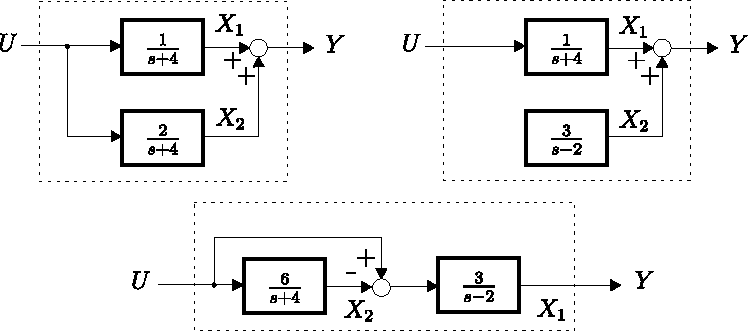
\includegraphics[width=0.8\columnwidth]{images/ZRD_nicht_steuerbare_systeme.pdf}
\end{center}


\subsubsection{Regelungsnormalform mittels Ähnlichkeitstransformation}

Ein steuerbares SISO-System kann mit einer geeigneten Transformationsmatrix $\bm{P}$ in Regelungsnormalform (siehe \ref{Regelungsnormalform}) 
gebracht werden. 


\begin{minipage}[c]{0.78\columnwidth}
    Diese geeigneten Transformationsmatrix $\bm{P}$ wird mittels folgendem Vorgehen ermittelt:

    \smallskip

    \begin{enumerate}
        \item Steuerbarkeitsmatrix $\bm{Q_S}$ invertieren   \\
            \textrightarrow\ Voraussetzung: muss invertierbar sein!
        \item Von $\bm{Q_S}^{-1}$ wird die letzte Zeile als $q$ bezeichnet
        \item Transformationsmatrix $\bm{P}$ bilden als
    \end{enumerate}
\end{minipage}
\hfill
\begin{minipage}[c]{0.2\columnwidth}
    $$
    \bm{P} =
    \begin{bmatrix}
        q                   \\
        q \cdot \bm{A}      \\
        q \cdot \bm{A}^2    \\
        \vdots              \\
        q \cdot \bm{A}^{n-1}
    \end{bmatrix}
    $$
\end{minipage}



\subsection{Beobachtbarkeit}{189}
\label{Beobachtbarkeit}

Die Beobachtbarkeit stellt die Frage danach, ob (bzw. wie) der \textbf{Zustand $\bm{x}$ durch die Messung des Ausgangs $\bm{y}$ bestimmt} werden kann.

\medskip

\paragraph{Defintionen von Beobachtbarkeit}

Beide Definitionen von Beobachtbarkeit sind äquivalent.

\smallskip

\begin{enumerate}
    \item Ein System $(\bm{A}, \bm{C})$ ist beobachtbar, wenn der Anfangszustand $x_0$ innert endlicher
        Zeit $T_e$ eindeutig bestimmt werden kann, sofern $u$ und $y$ für $0 \leq t \leq T_e$ bekannt sind.
    \item Ein System $(\bm{A}, \bm{C})$ ist beobachtbar, wenn die Eigenwerte von $\bm{A} - \bm{HC}$ durch geeignete
        Wahl von $\bm{H}$ beliebig plaziert werden können.
\end{enumerate}



\subsubsection{Beobachtbarkeitsmatrix $\bm{Q_B}$}
\label{Beobachtbarkeitsmatrix}

Ein System ist \textbf{vollständig beobachtbar}, wenn

\begin{outline}
    \1 Der \textbf{Rang} der Beobachtbarkeitsmatrix $\bm{Q_B}$ der Ordnung $n$ des Systems entspricht
        \2 Die Matrix $\bm{Q_B}$ hat somit vollen Rang
    \1 Bei Single-Output-System:  Die \textbf{Determinante} von $\bm{Q_B}$ \textbf{ungleich Null ist}
\end{outline}

\smallskip

\begin{minipage}[c]{0.4\columnwidth}
    $$
    \bm{Q}_B = 
    \begin{bmatrix}
        \bm{C} \\ \bm{C A} \\ \bm{C A^2} \\ \vdots \\ \bm{C A^{n-1}} 
    \end{bmatrix}
    $$
\end{minipage}
\hfill
\begin{minipage}[c]{0.58\columnwidth}
    \begin{tabular}{ll}
        Dimension:  & $(k \cdot n) \times n$ \\
        $\bm{A}$    & Systemmatrix ($n \times n$) \\
        $\bm{C}$    & Beobachtungsmatrix ($k \times m$) \\
        $n$         & Zustände \\
        $m$         & Eingänge \\
        $k$         & Ausgänge 
    \end{tabular}
\end{minipage}


\subsubsection{Nicht-beobachtbare Systeme}

\begin{outline}
    \1 Gewisse Eigenwerte von $\bm{A} - \bm{HC}$ sind \textbf{nicht verschiebbar}
    \1 Anzahl der fixen Eigenwerte entspricht dem Defizit des Rangs von $\bm{Q_B}$
\end{outline}


\example{Typische nicht-beobachtbare Systeme}

\begin{center}
    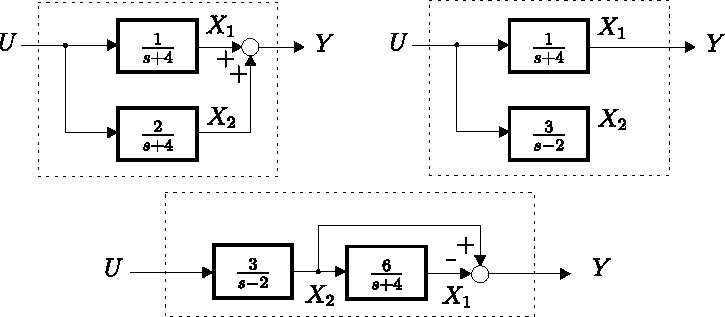
\includegraphics[width=0.8\columnwidth]{images/ZRD_nicht_beobachtbare_systeme.pdf}
\end{center}


\subsection{Minimalität}

Ein System ist minimal, wenn...
\begin{outline}
    \1 Das System \textbf{steuerbar und beobachtbar} ist
    \1 Keine Pol-/NS-Kürzungen in der UTF möglich sind
\end{outline}

% Ist ein System \textbf{steuerbar und beobachtbar}, so ist es minimal. In der UTF können keine Pol-/NS-Kürzungen vorgenommen werden.

\smallskip

Zu einem nicht-minimalen System $(\bm{A}, \, \bm{B}, \, \bm{C})$ kann ein System $(\bm{A_M}, \, \bm{B_M}, \, \bm{C_M})$ tieferer Ordnung
angegeben werden, das trotzdem \textbf{dieselbe UTF}(-Matrix) $G(s)$ hat.

\subsubsection{Einfluss von Nichtminimalität}

\begin{outline}
    \1 \textbf{Bau eines neuen Systems}
        \2 Ersetzung durch minimale Version des Systems \\
        \textrightarrow\ Bau der \textbf{minimale Realisierung} des Systems
    \1 \textbf{Reglerentwurf für bestehende nichtminimale Strecke}
        \2 mindestens ein Pol (bzw. Eigenwert) der Strecke nicht veränderbar \\
            \textrightarrow\ \textbf{gravierend}, wenn Strecke deshalb nicht stabilisiert werden kann
        \2 Algorithmen / Softwarepakete funktionieren oft nicht korrekt, wenn System nicht minimal
\end{outline}



\subsection{Normalformen}

Kann ein SISO-System mit UTF $G(s)$ in eine der beschriebenen Normalformen gebracht werden, so hat das System gewisse Eigenschaften

$$  G(s) = d + \frac{b_{n-1} s^{n-1} + \cdots + b_1 s + b_0}{s^n + a_{n-1} s^{n-1} + \cdots + a_1 s +a_0 } $$


\subsubsection{Regelungsnormalform}{188}
\label{Regelungsnormalform}

Kann ein System in Regelungsnormalform gebracht werden, so ist es \textbf{immer steuerbar}.

$$
A =
\begin{bmatrix}
    0       & 1         & 0         & \cdots    & 0         \\
    0       & 0         & 1         & \ddots    & \vdots    \\
    \vdots  &           & \ddots    & \ddots    & \vdots    \\
    0       & 0         & \cdots   & 0         & 1         \\
    -a_0    & -a_1      & \cdots    & -a_{n-2}  & -a_{n-1}
\end{bmatrix}
\quad
b =
\begin{bmatrix}
    0 \\ 0 \\ \vdots \\ 0 \\ 1
\end{bmatrix}
\quad
c =
\begin{bmatrix}
    b_0 \\ b_1 \\ \vdots \\ b_{n-2} \\ b_{n-1}
\end{bmatrix}^{T}
\quad
d = d
$$



\subsubsection{Beobachtungsnormalform}

Kann ein System in Beobachtungsnormalform gebracht werden, so ist es \textbf{immer beobachtbar}.

$$
A =
\begin{bmatrix}
    0       & 0         & 0         & \cdots    & -a_0      \\
    1       & 0         & 0         & \cdots    & -a_1      \\
    0       & 1         & \ddots    & \ddots    & \vdots    \\
    \vdots  & \ddots    & \ddots    & 0         & -a_{n-2}  \\
    0       & \cdots    & 0         & 1         & -a_{n-1}
\end{bmatrix}
\quad
b =
\begin{bmatrix}
    b_0 \\ b_1 \\ \vdots \\ b_{n-2} \\ b_{n-1}
\end{bmatrix}
\quad
c =
\begin{bmatrix}
    0 \\ 0 \\ \vdots \\ 0 \\ 1
\end{bmatrix}^{T}
\quad
d = d
$$

\textbf{Hinweis:} Die Beobachtungsnormalform ist \textbf{dual} zur Regelungsnormalform.


\subsection{Eigenschaften von Zustandsraummodellen}{190-193}

Ausgewählte wichtige Eigenschaften eines Systems $(\bm{A}, \bm{B}, \bm{C})$ mit Zustandsvektor $x$ sind hier noch einmal aufgelistet:

\smallskip

\begin{outline}
    \1 Die Ordnung des Systems entspricht der Länge des Zustandsvektors $x$
    \1 System ist asymptotisch stabil, wenn alle Eigenwerte von $\bm{A}$ in der LHE liegen bzw. alle
        $\lambda_i < 0$ sind 
    \1 System ist steuerbar, wenn $\bm{Q_S}$ vollen Rang hat
    \1 System ist beobachtbar, wenn $\bm{Q_B}$ vollen Rang hat
        \2 Bei einem Beobachtbarkeits-Problem kann z.B. ein zusätzlicher Sensor die Strecke beobachtbar machen
    \1 Ein System ist minimal, wenn es steuerbar \textbf{und} beobachtbar ist
    \1 Wenn nur die UTF $G(s)$ eines Systems bekannt ist, sind \textbf{keine Aussagen über Steuerbarkeit / Beobachtbarkeit möglich} \\
        \textrightarrow\ Dafür muss innerer Aufbau des Systems (ZRD) bekannt sein!
\end{outline}



